\chapter{SCV Reference manual}
\section{Introduction and Purpose}
Source Cleaning Vessel (SCV) is an apparatus for the cleaning of calibration sources and comprises a cylindrical tube, plugs, flanges, conical base and spray nozzles. The central part of the vessel is made up of a  cylindrical tube and connected with the top and bottom parts through the flanges. The nozzles from top and bottom uniformly sprays the lab on the source for essential cleaning and the drain port in the base provides access for collecting the sample for testing. The following document describes all the information regarding the SCV and its related parts, apart from that it also provides hyperlinks to references and suppliers. Figure~\ref{fig:SCV} depicts its dimension and associated parts.
\begin{figure}[!htpb]
  \centering
  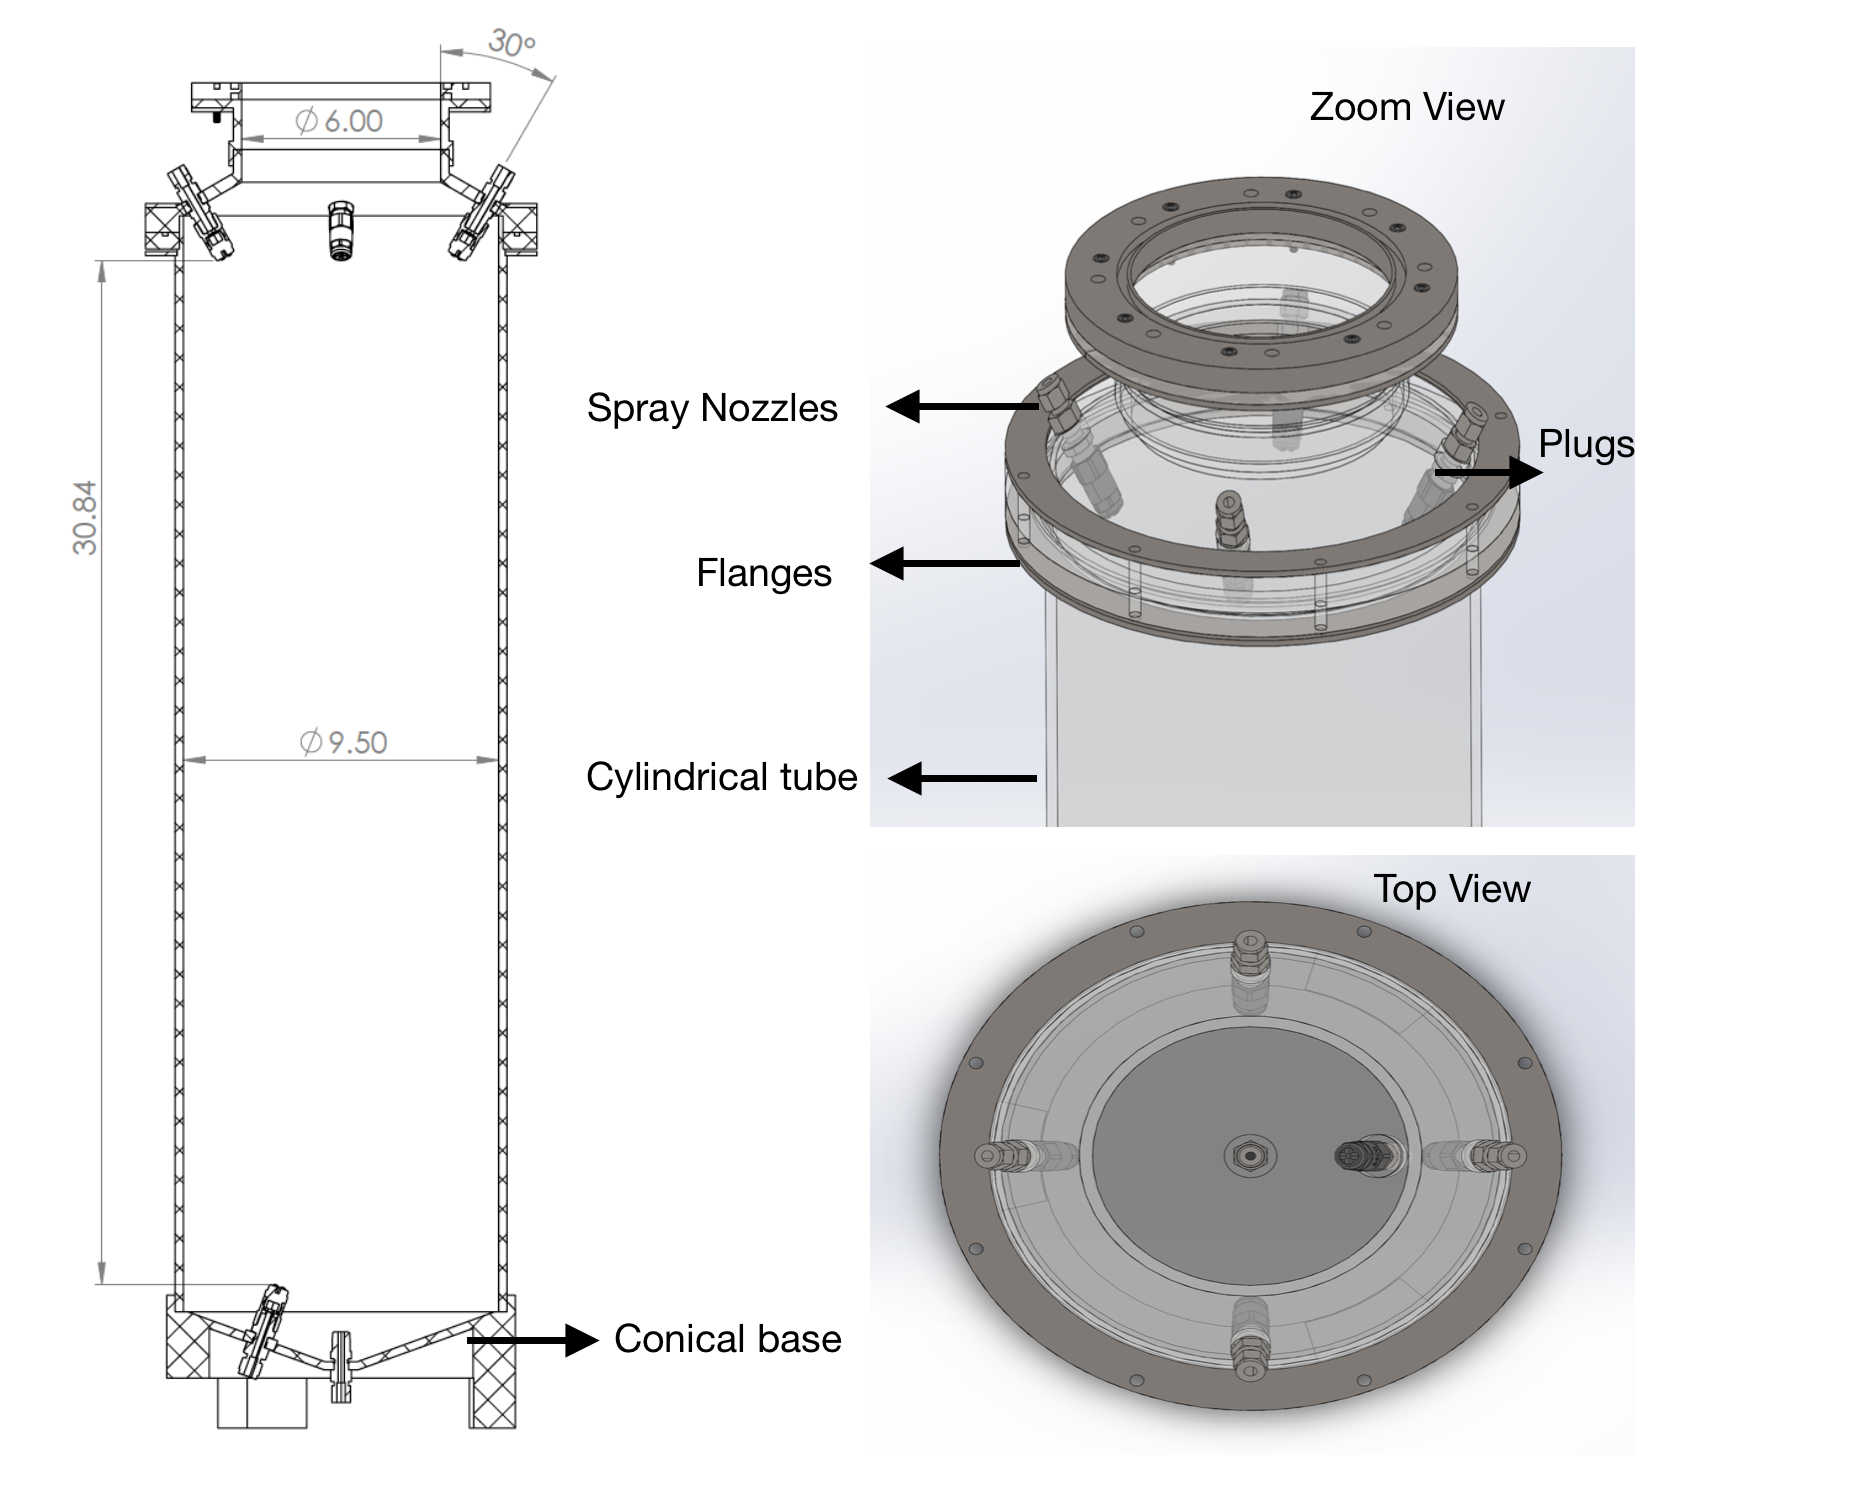
\includegraphics[width = 12cm, height=7cm ]{figures/SCV}
  \caption{Source Cleaning Vessel}
  \label{fig:SCV}
\end{figure}

\section{ Definitions and Parts of SCV}

\textbf{Cylindrical tube}: \\
It embodies the central part of the vessel that accommodates the source.\\
\\
Purchased From: Johnston industrial plastics limited\\
\\
Link:  \url{https://www.johnstonplastics.com}\\
\\
Dimension for the vessel: 9.50$''$(ID) x 0.25$''$Thickness) x 30.84$''$(Length).\\
\\
Material: Cast Acrylic.\\
\\
**I will add a picture when going back to the lab.\\
\\
\textbf{Plugs}:\\
These are small circular hollow discs used with bulkhead fitting to connect spray nozzles.\\
\\
\begin{figure}[!htpb]
  \centering
  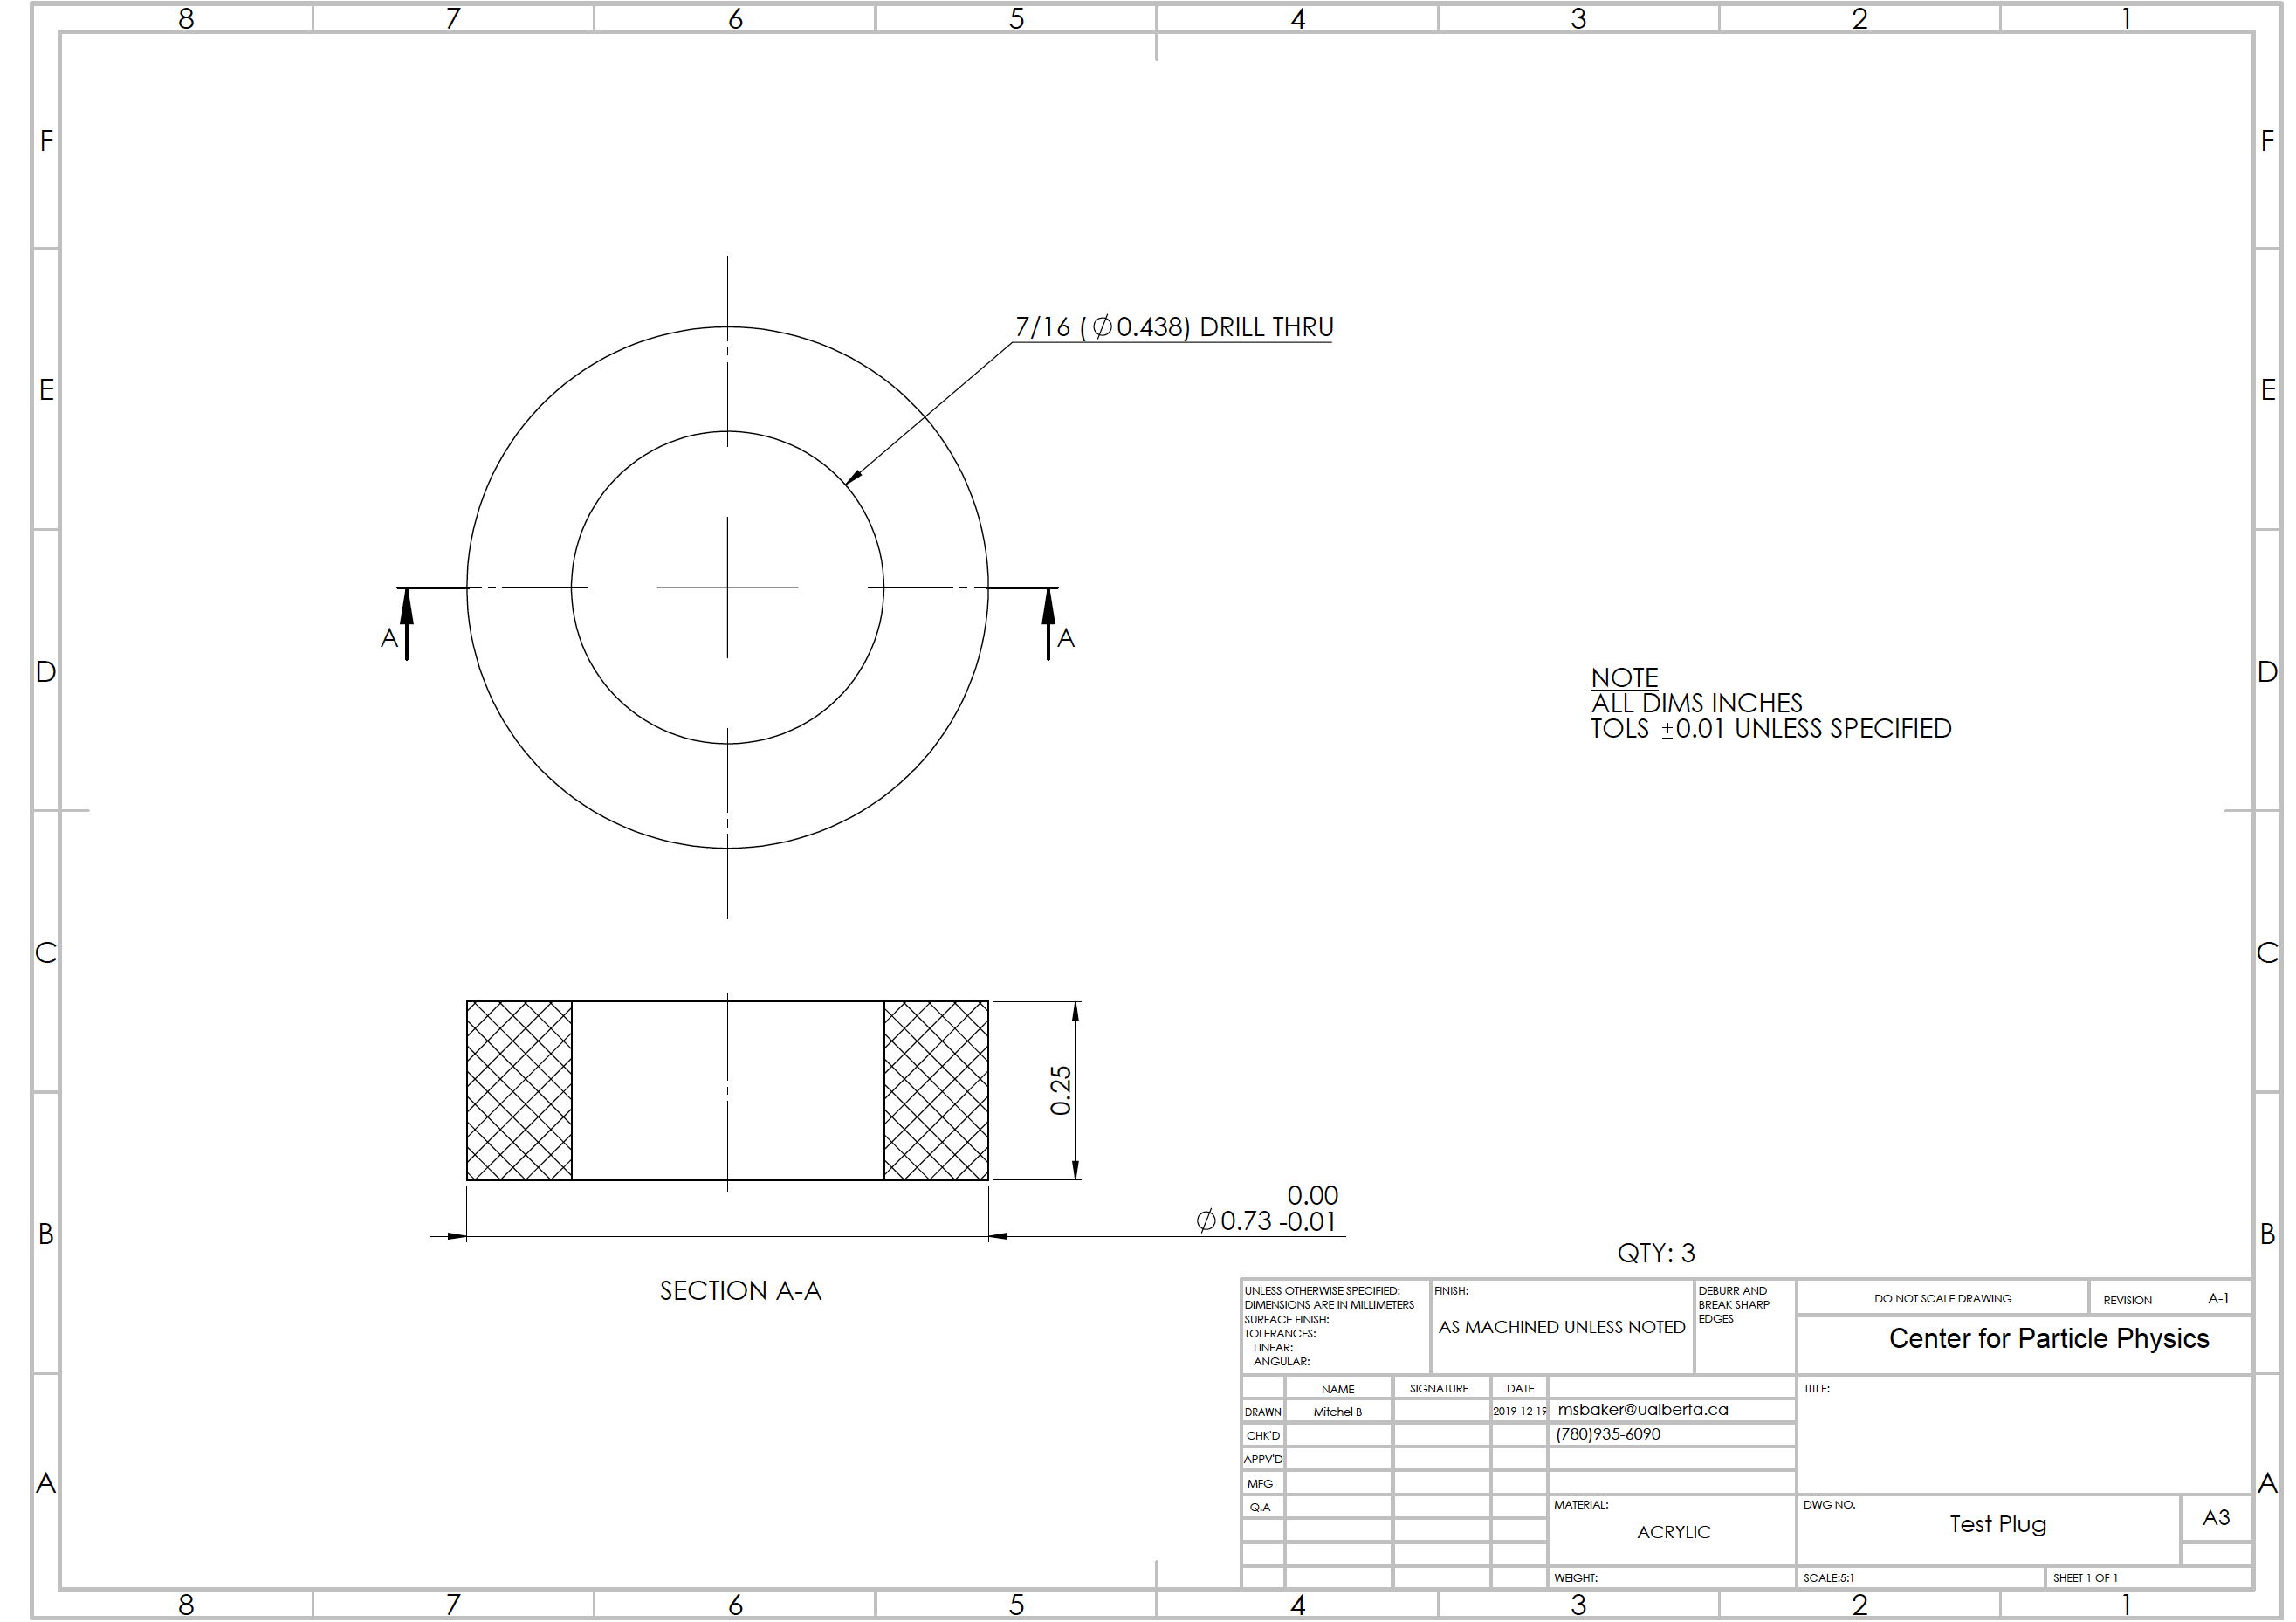
\includegraphics[width = 12cm, height=10cm ]{figures/plug}
  \caption{Drawing corresponding to plug}
  \label{fig:plug}
\end{figure}
\\
Dimension: 0.43$''$(ID) x 0.25$''$(Thickness) x 0.73$''$(Length).\\
\\
Material: Acrylic ( Rod from physics workshop)\\
\\
\begin{figure}[!htpb]
  \centering
  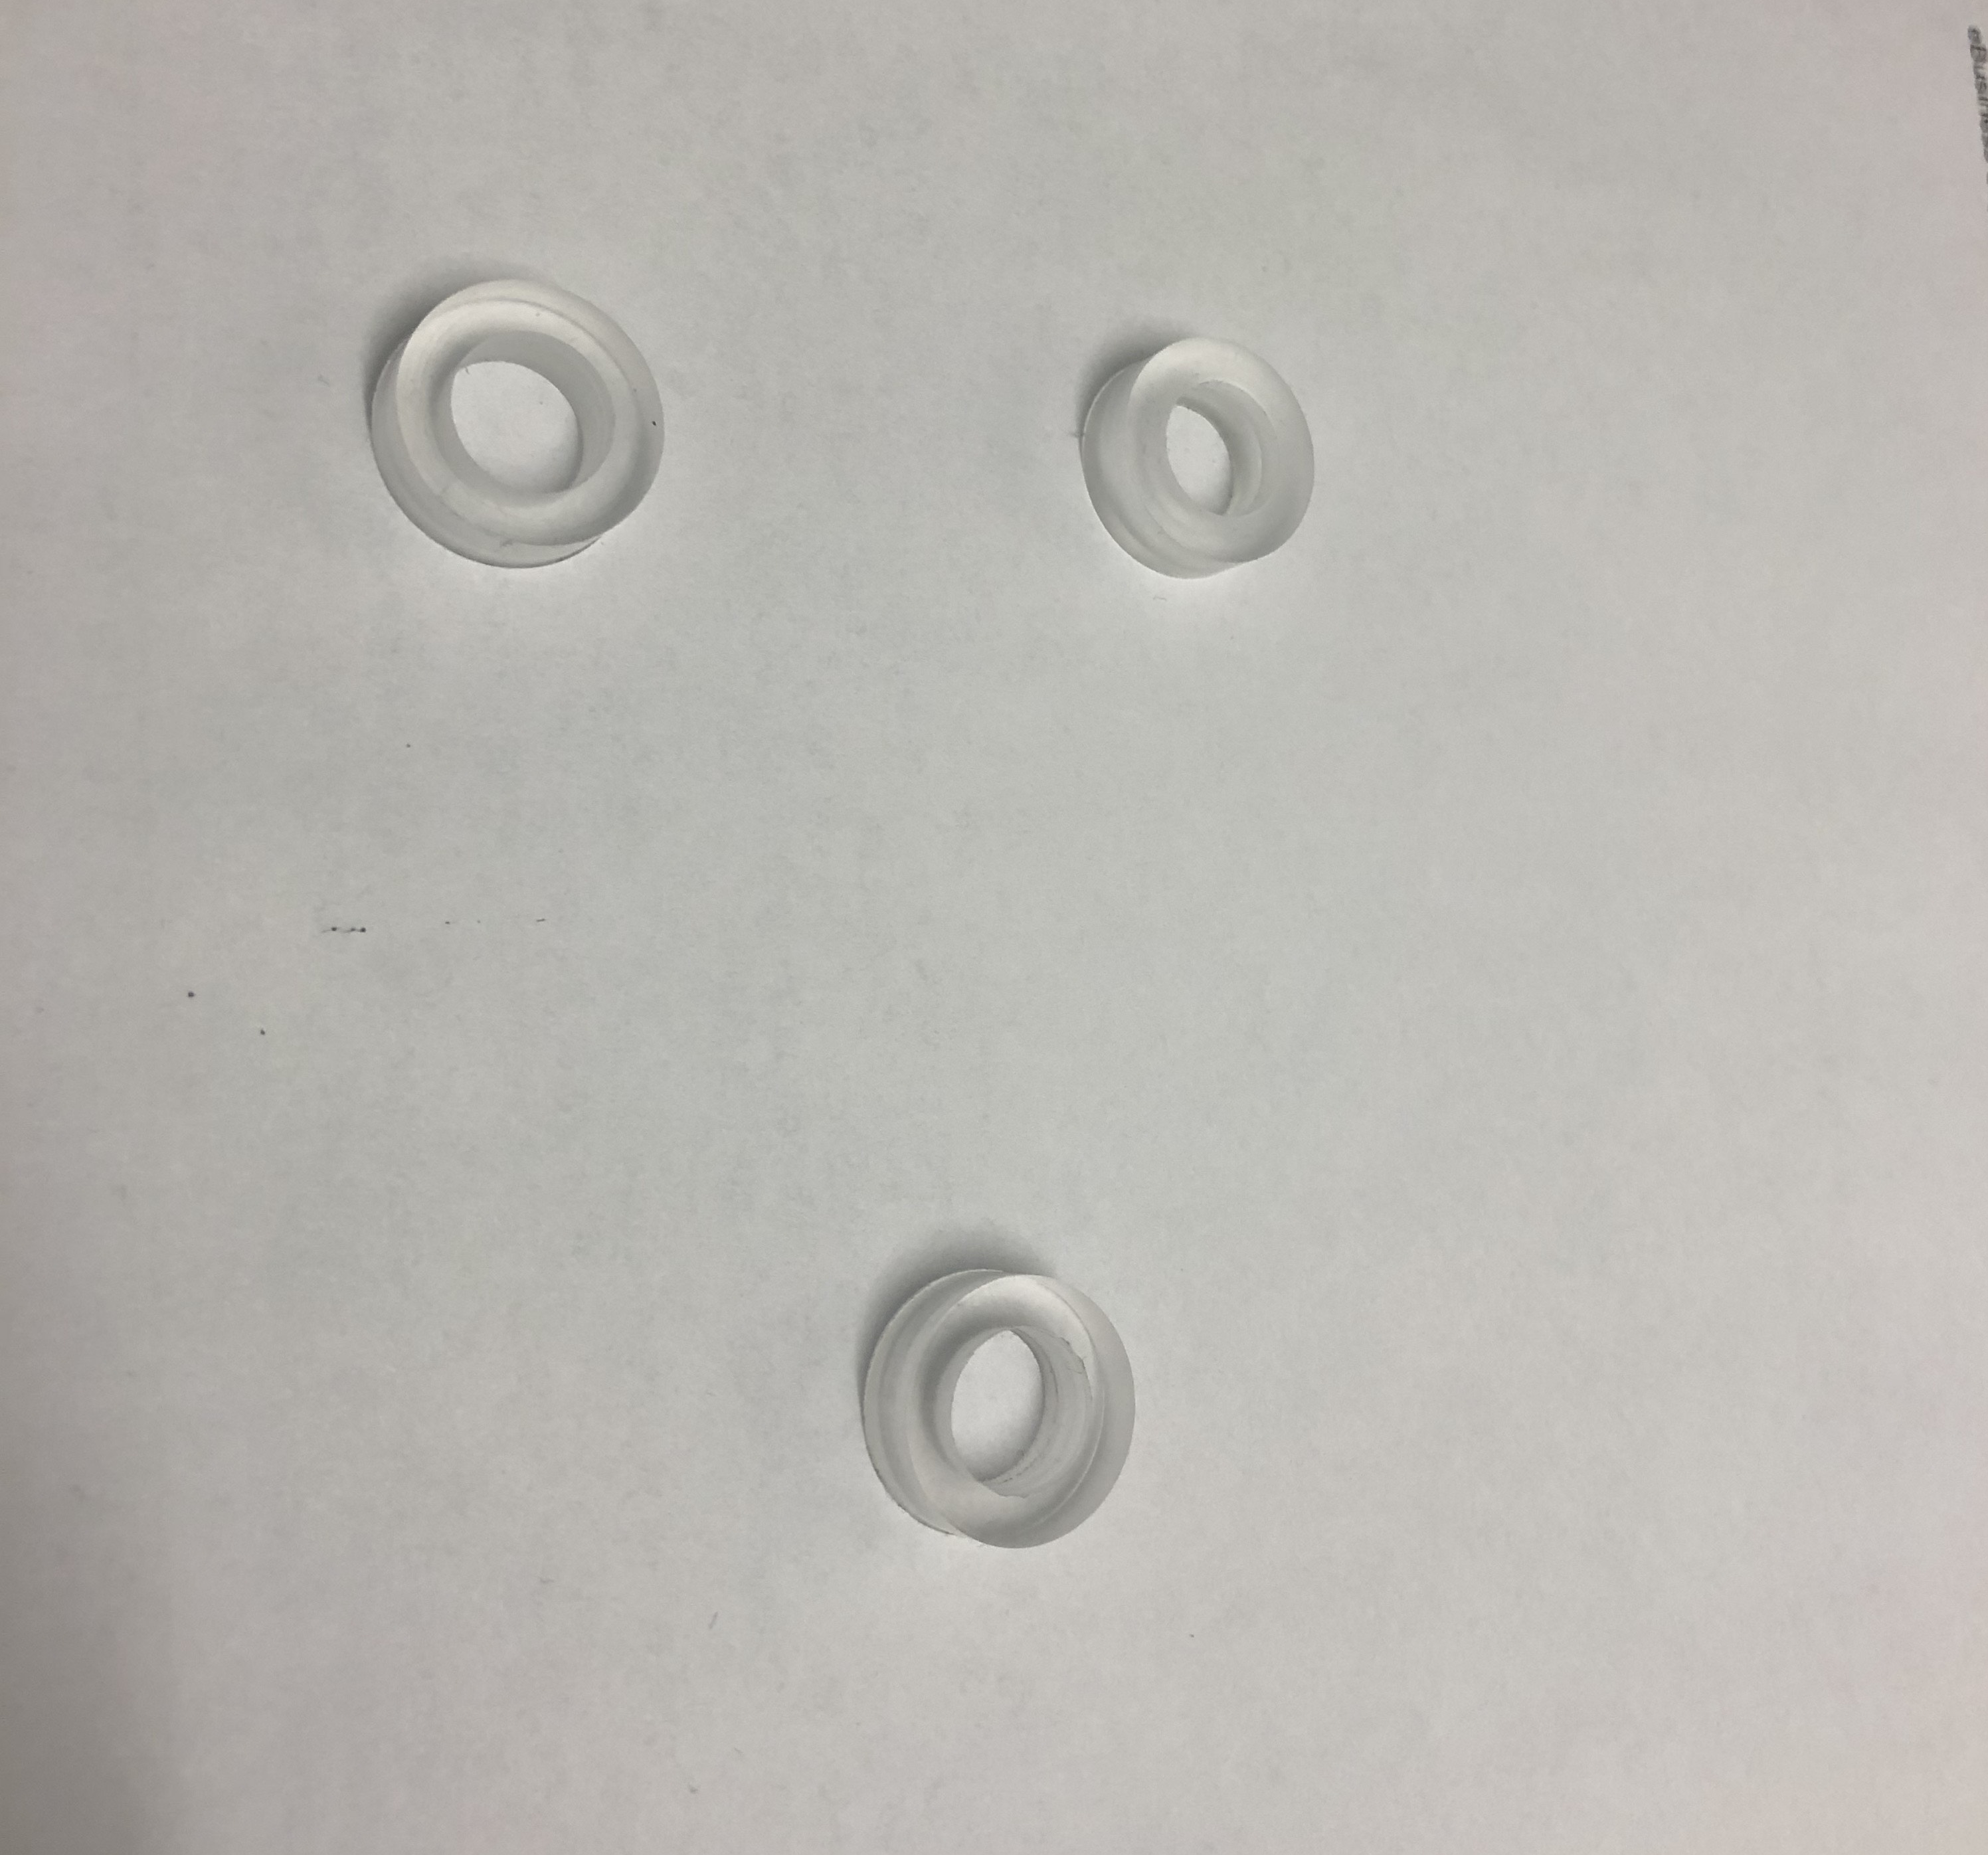
\includegraphics[width = 7cm, height=6cm ]{figures/plug1}
  %
   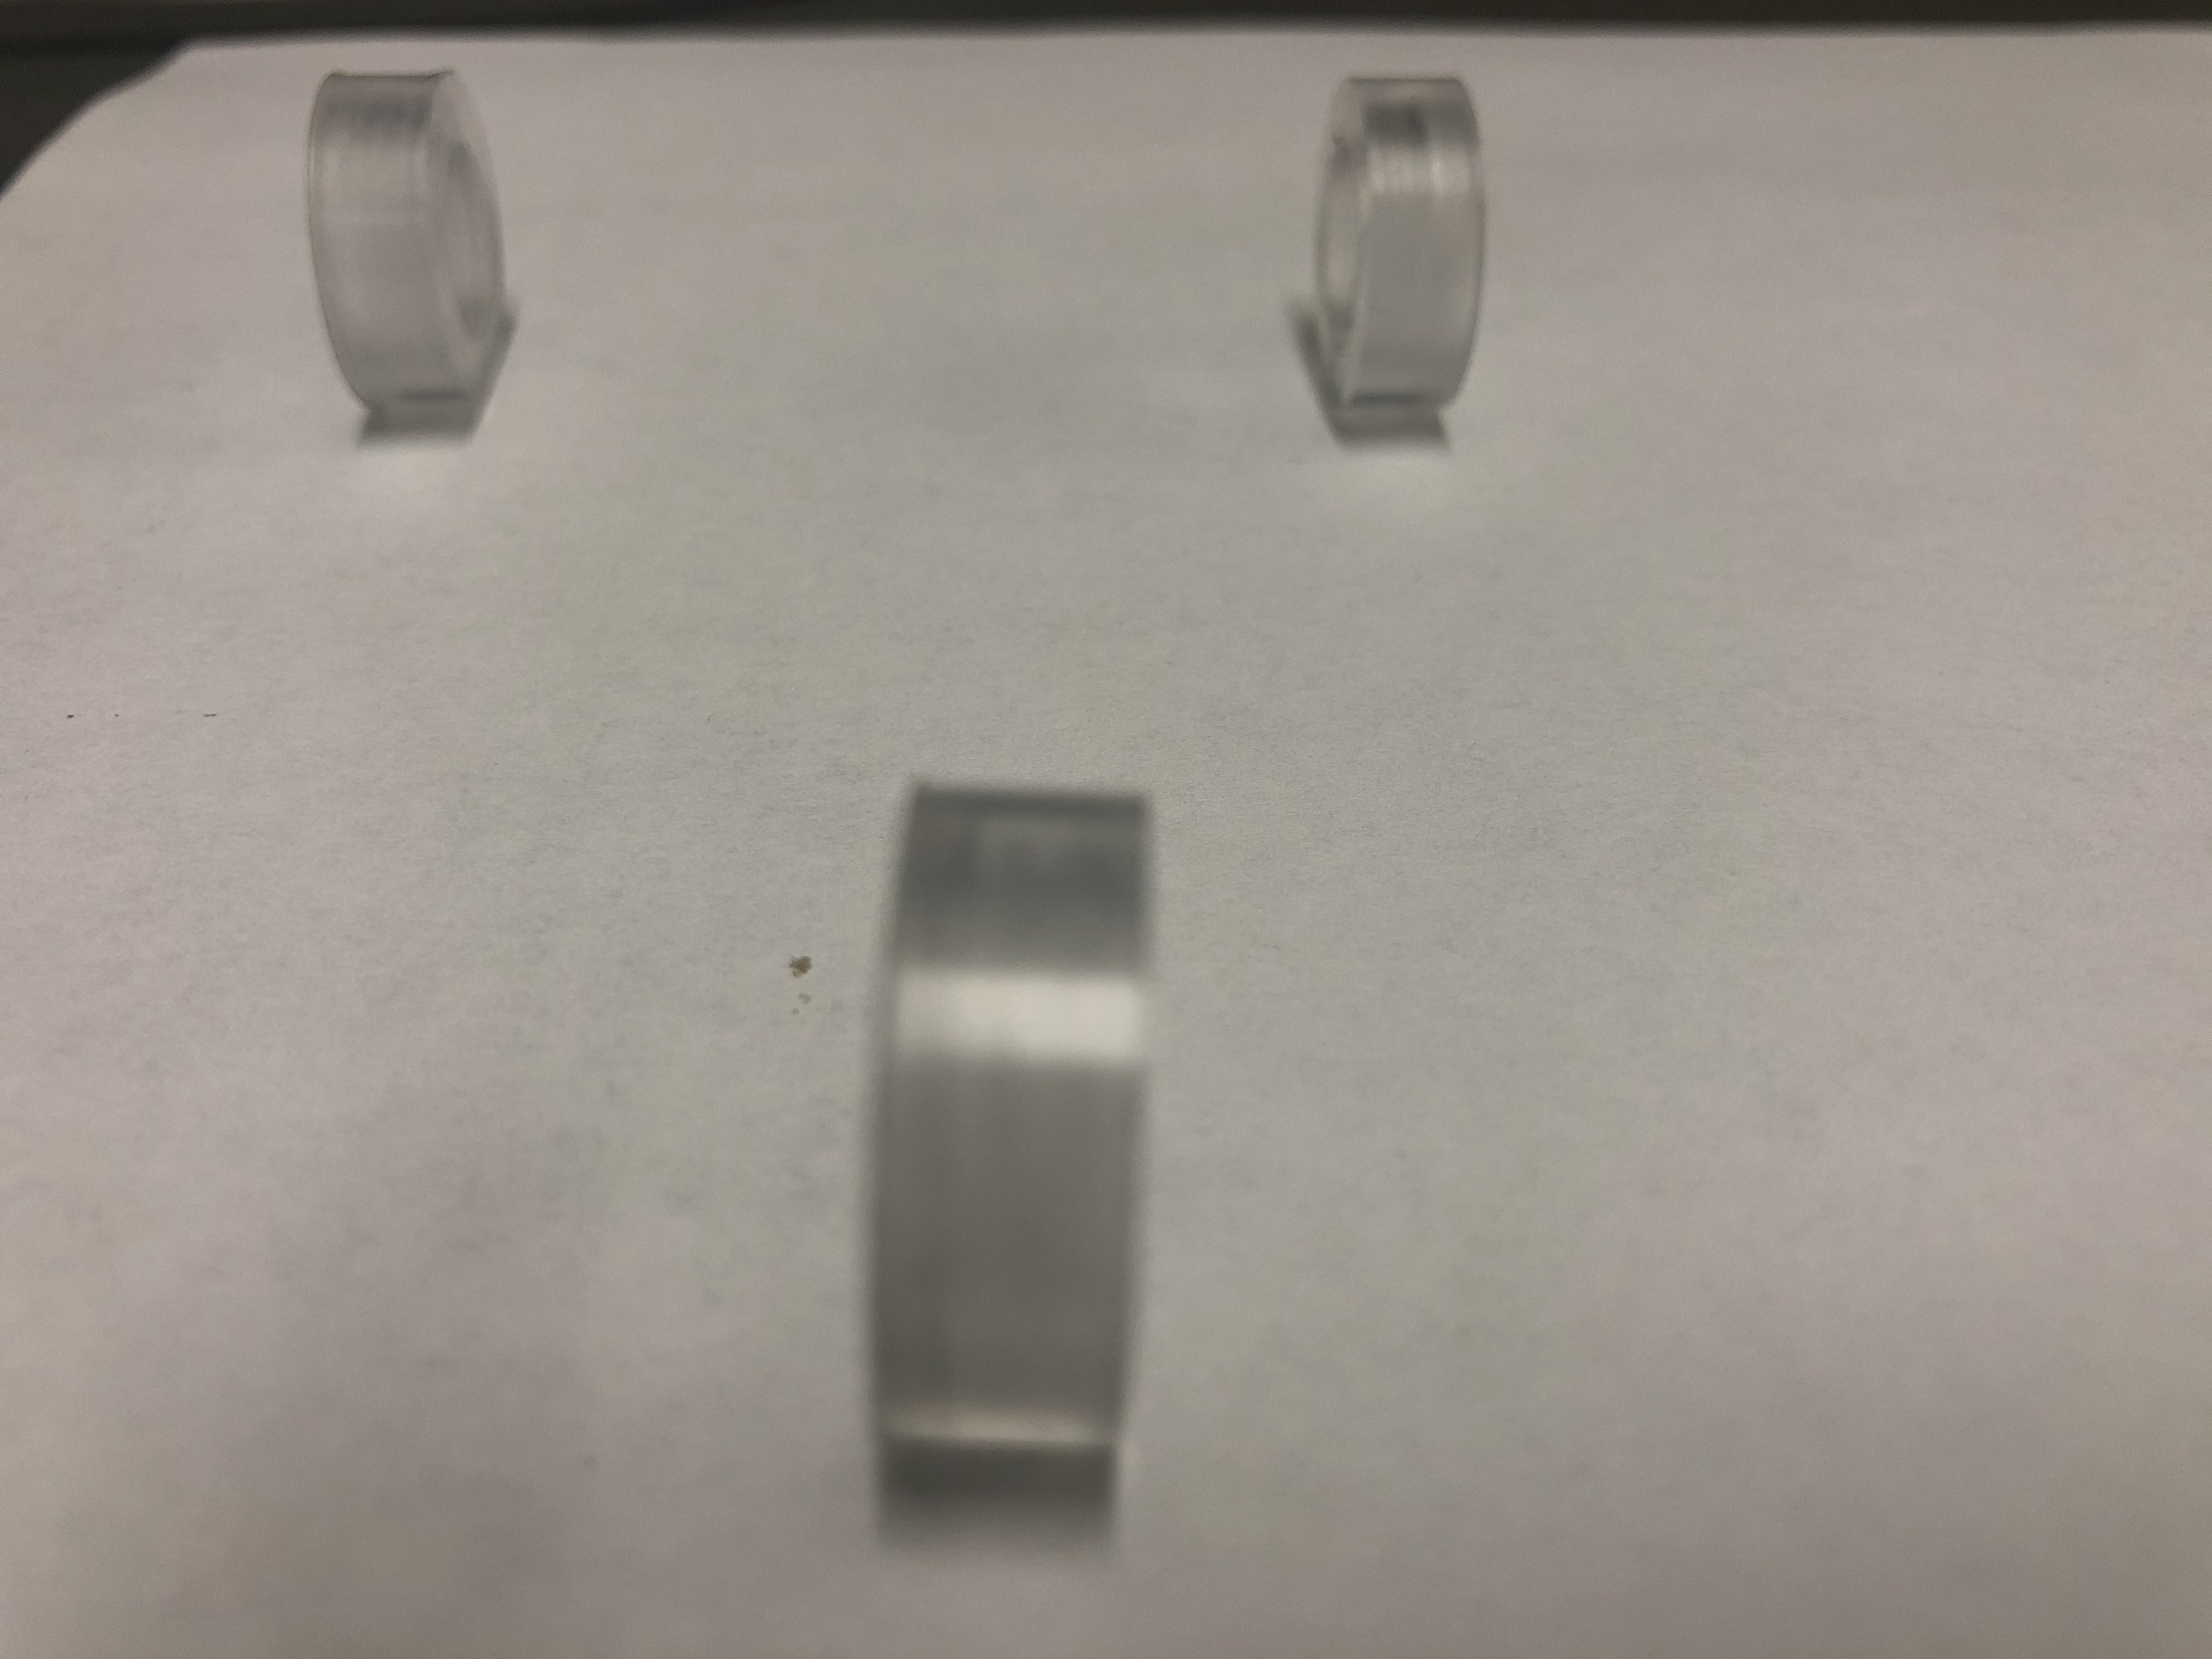
\includegraphics[width = 7cm, height=6cm ]{figures/plug2}
  \caption{Plugs for bulkhead fittings}
  \label{fig:plug1}
\end{figure}
\\
\textbf{Flanges}:
These are large hollow discs used to bond different SCV parts and provide accessibility to the other components of the vessel.  
\\
Dimension: 9.75$''$(ID) x 0.50$''$ (Thickness) x 11.80$''$(Length).\\
\\
Material: Acrylic ( Acrylic sheet from lab L2-92)\\
\begin{figure}[!htpb]
  \centering
  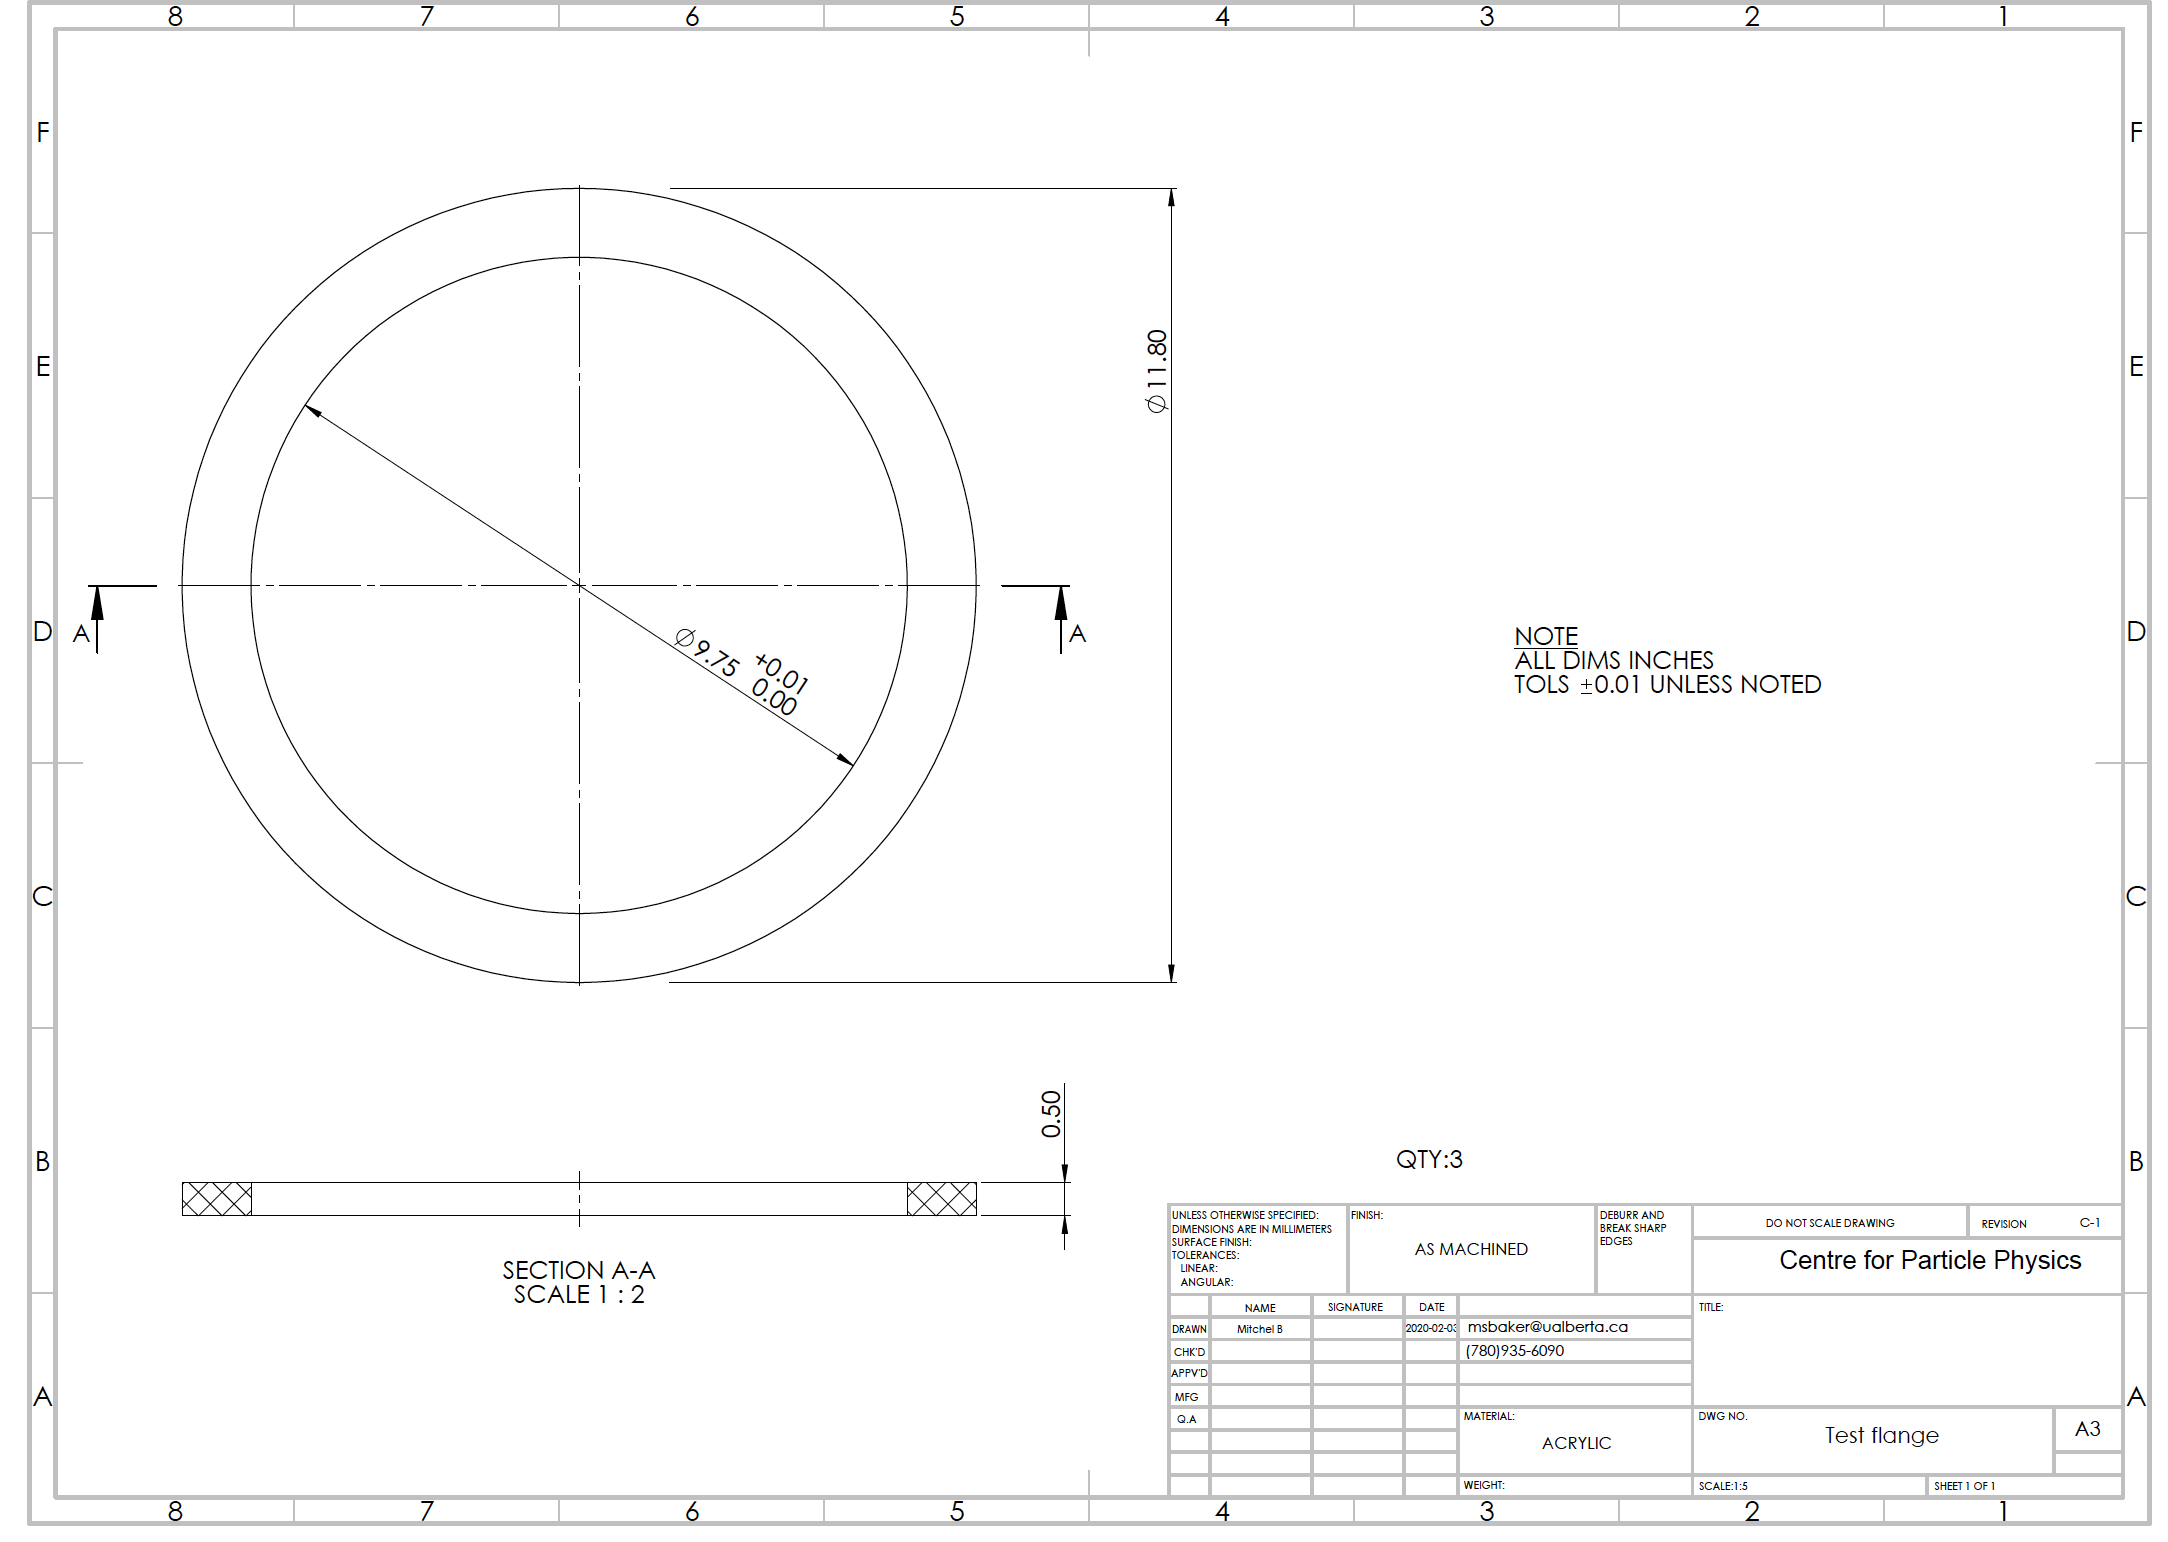
\includegraphics[width = 12cm, height=10cm ]{figures/flange}
  \caption{Drawing corresponding to flange}
  \label{fig:flange}
\end{figure}

In our design we are using two types of flanges:\\

Permanent \\

Removable\\

The purpose of the permanent flanges is to join together the components that are made of different pieces of acrylic.  For example, the bottom cone has to be bonded to the tube.  Also, the top nozzle adapter (also cone-shaped) has to be bonded to the flange adapter.  The reason we don’t just make those two pieces as a single unit is that the raw material comes in sheets with a maximum thickness of 4 inches.  The purpose of  removable (the one close to the upper nozzles) is to allow access to the nozzles in the future, in case they need to be cleaned or replaced.  The top flange connects to the gate valve on the Umbilical Retrieval Mechanism (URM).
\begin{figure}[!htpb]
  \centering
  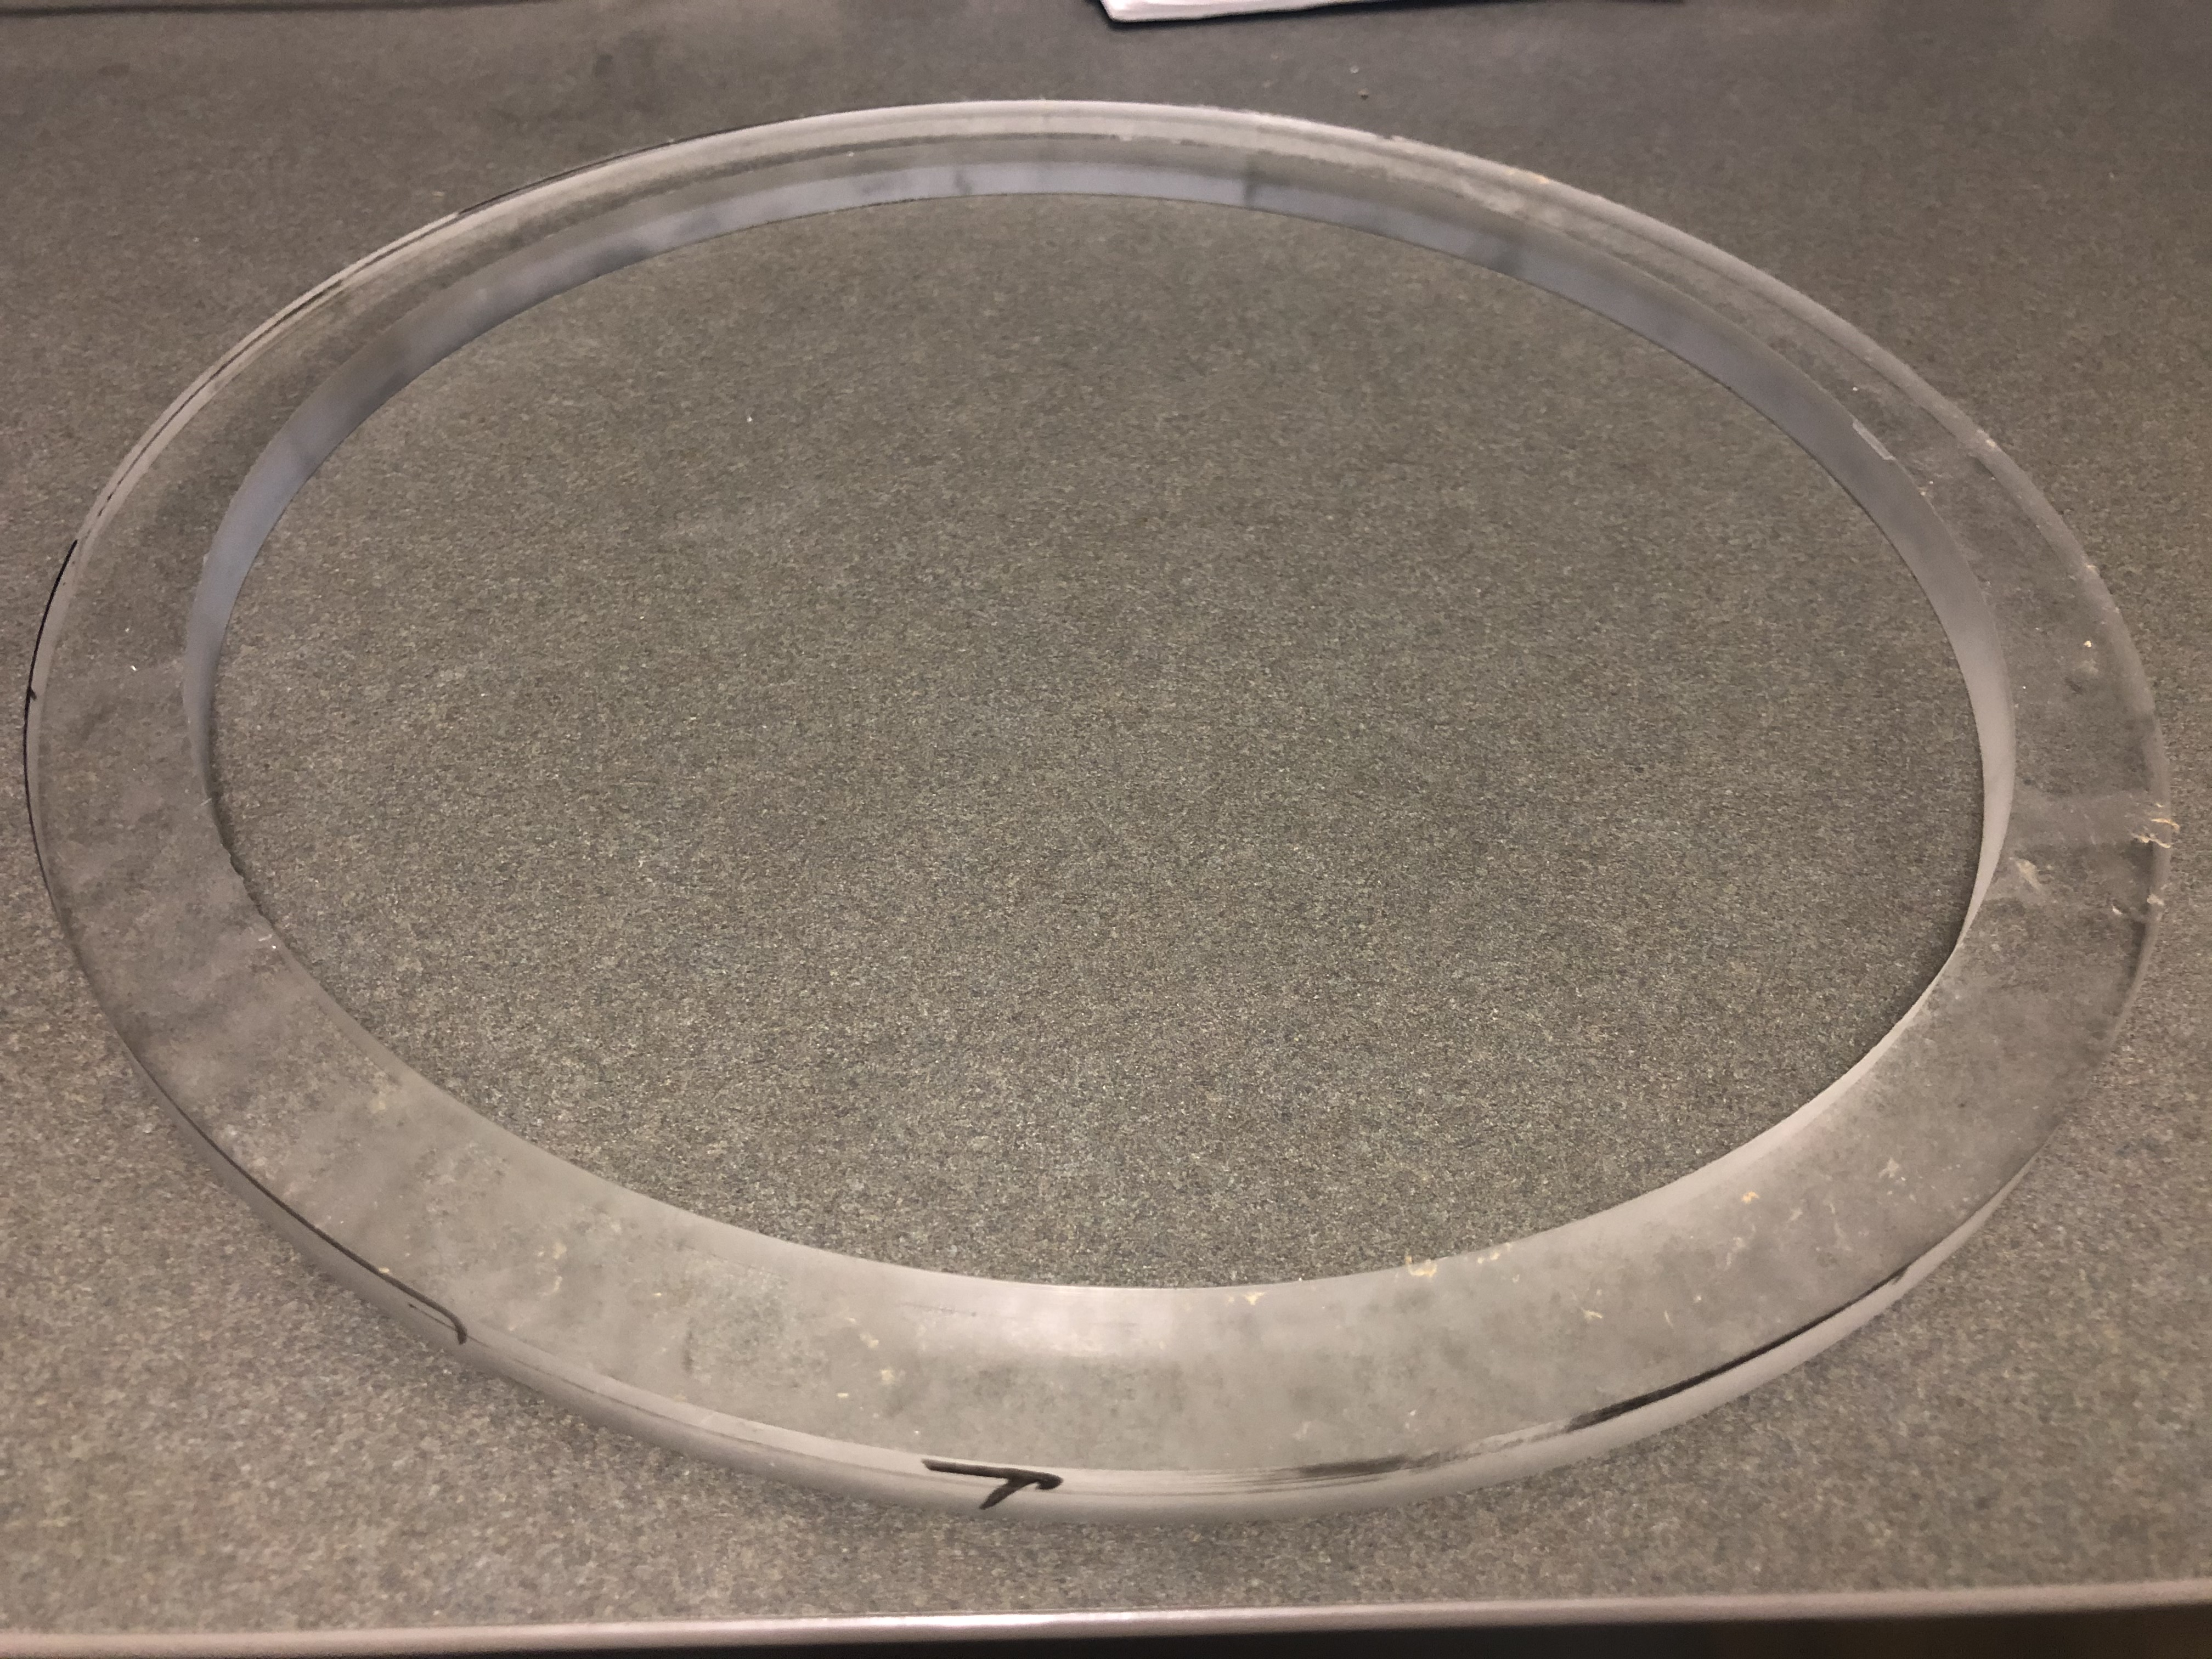
\includegraphics[width = 7cm, height=6cm ]{figures/flange1}
  \caption{Flange for connection of different parts}
  \label{fig:flange1}
\end{figure}
\\
\\
\textbf{Conical Base}:
It is the bottom part of the vessel with a conical shape and provides a drainage port to collect Lab samples for testing. The conical geometry allows the used cleaning fluid to drain out of the vessel without leaving dirty fluid behind.
\\
Material: Acrylic(Acrylic sheet from physics lab)\\
** I will add a picture of the machined part and update this drawing with the final version when we go back to the lab.\\
\begin{figure}[!htpb]
  \centering
  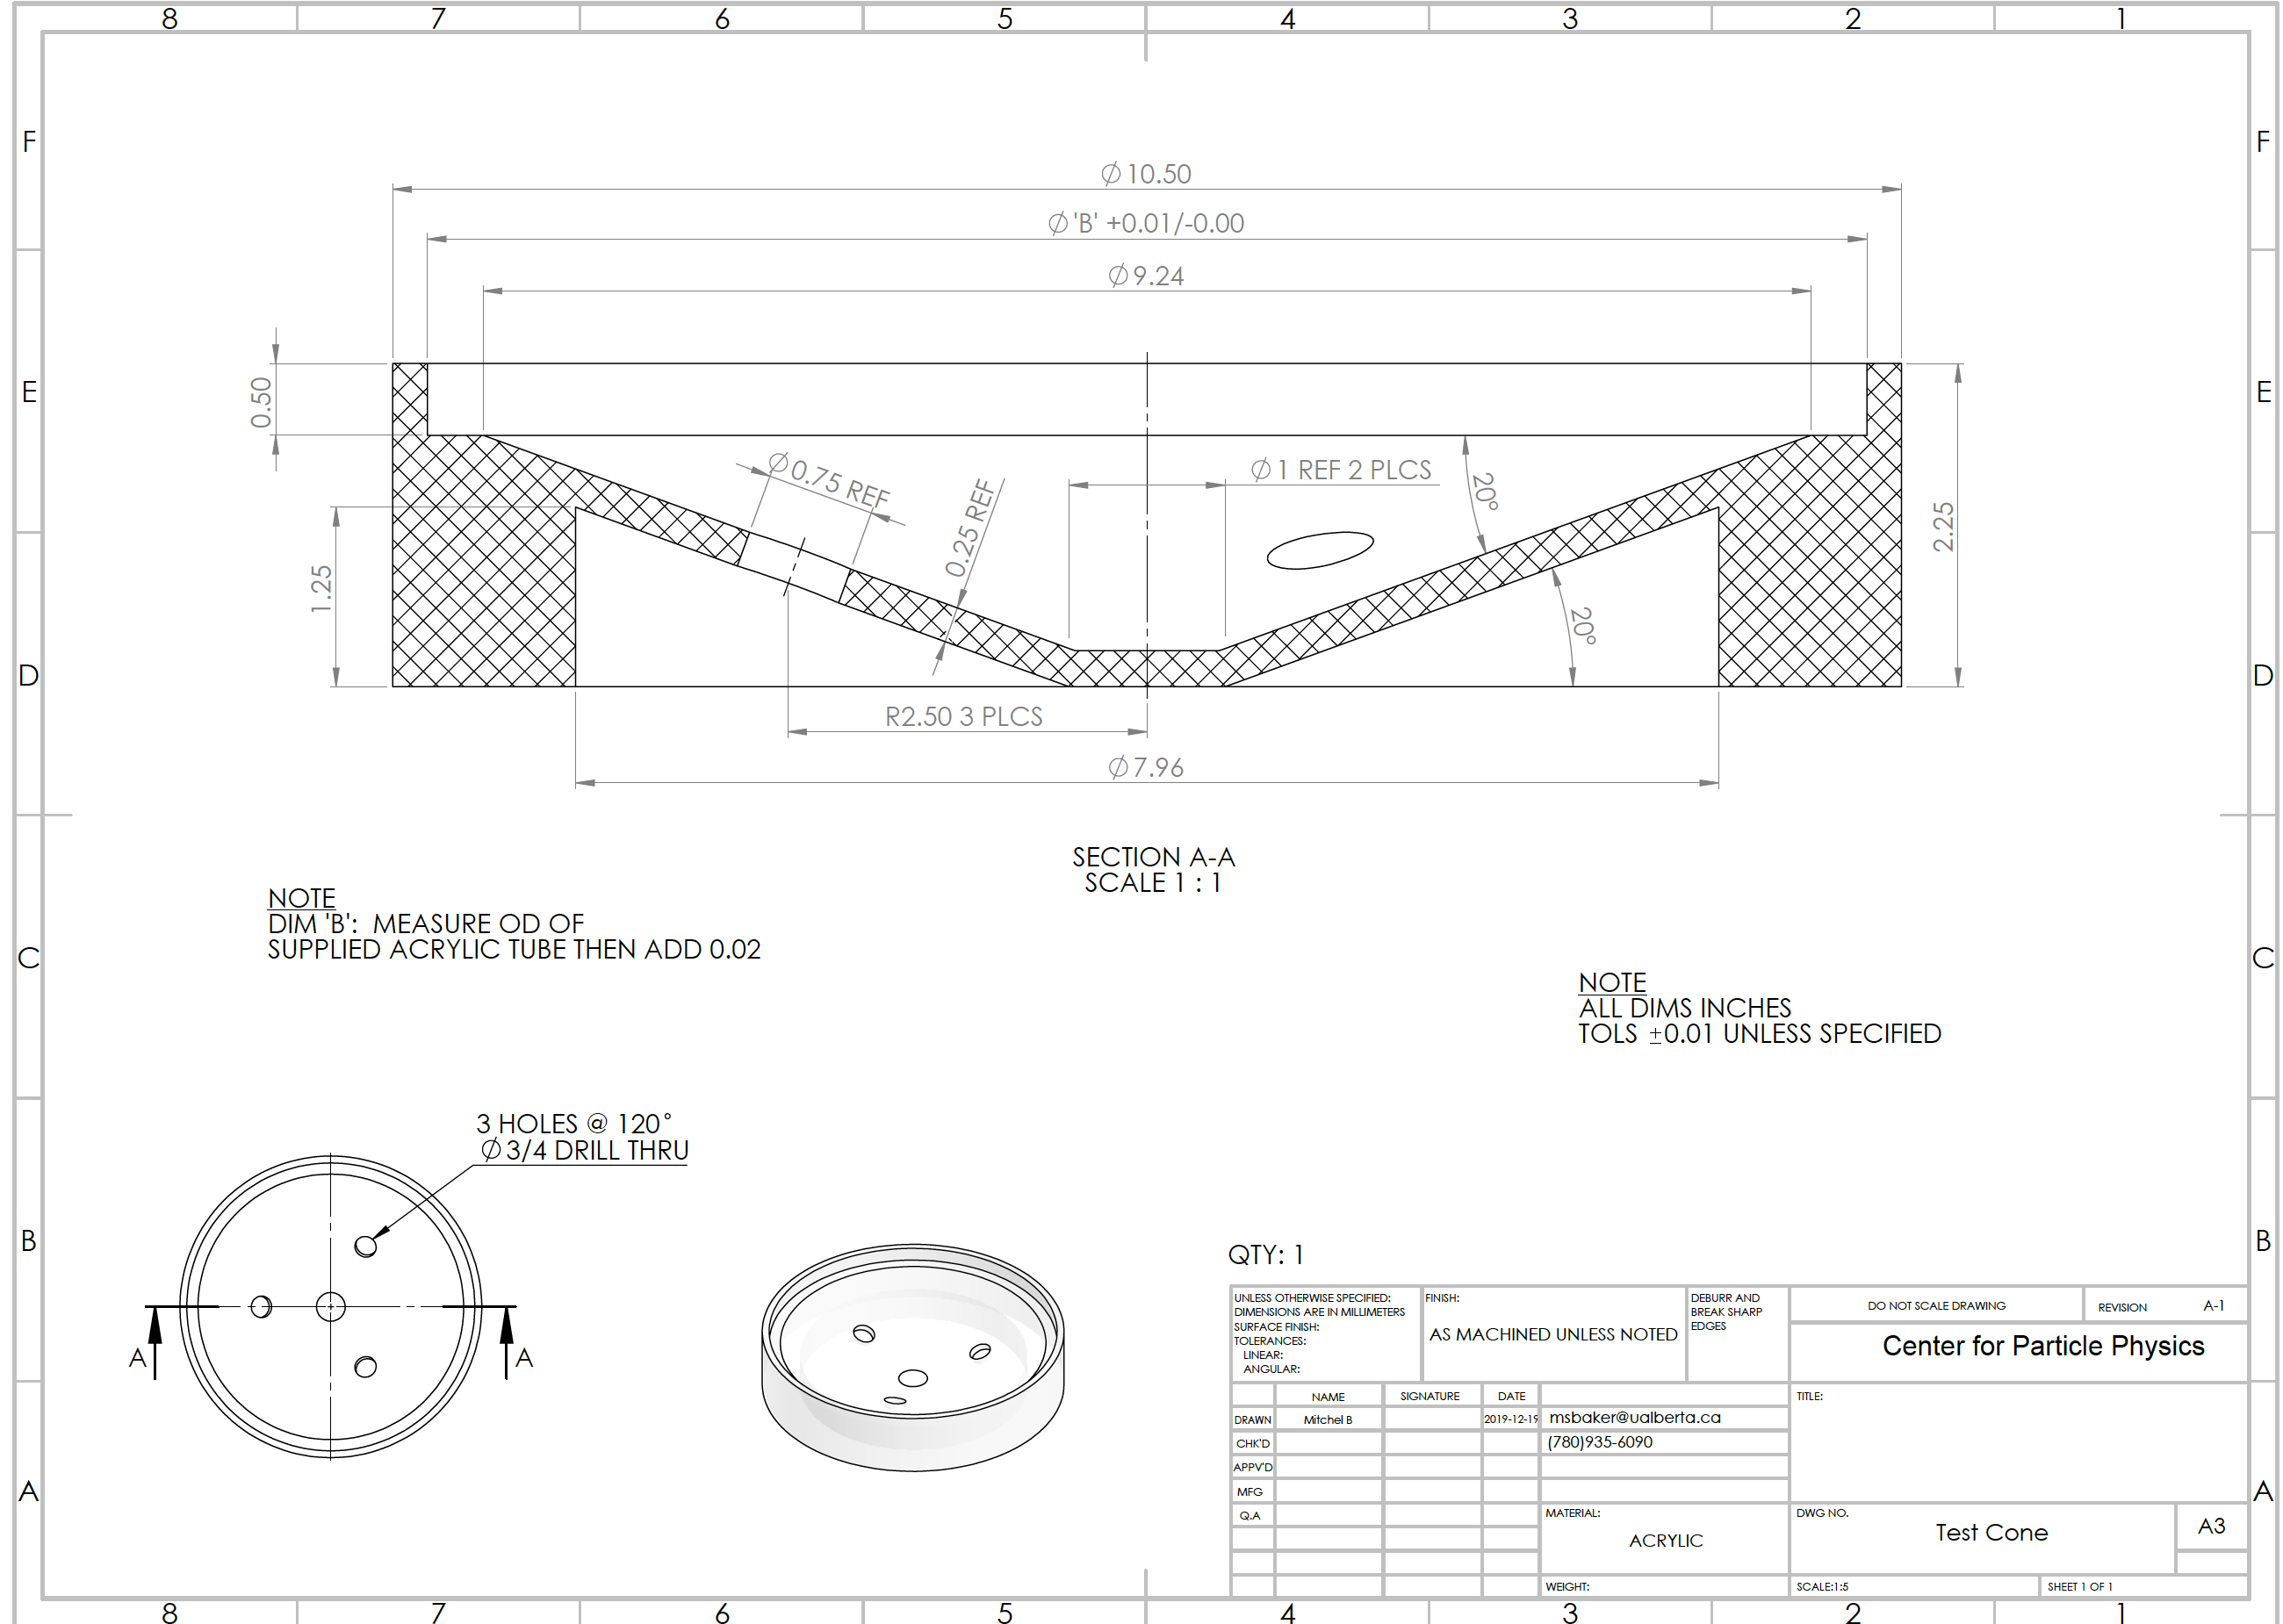
\includegraphics[width = 12cm, height=10cm ]{figures/base}
  \caption{Drawing corresponding to Conical base}
  \label{fig:base}
\end{figure}
\\
\textbf{Spray Nozzles}:
Spray nozzle is a simple device used to break apart a fluid flow into a spray pattern. It is one of the crucial parts of any cleaning system and needs to be chosen appropriately for the effective cleaning. There are many variables that should be explored and investigated before the selection of suitable nozzles for any cleaning system. The variables are as follow:\\

\textbf{Dust particle size} \\                                              

\textbf{Spray drop size}\\

\textbf{Spray pattern}\\

\textbf{Spray angle}\\

\textbf{Operating pressure}\\

\textbf{Nozzle placement}\\
\\
Keeping in mind these requirements and after exploring all the variables according to the need of our system, we have chosen Full cone wide-angle ( 112 and 120 deg) hydraulic nozzles(Figure~\ref{fig:nzl}).\\

\begin{figure}[!htpb]
  \centering
  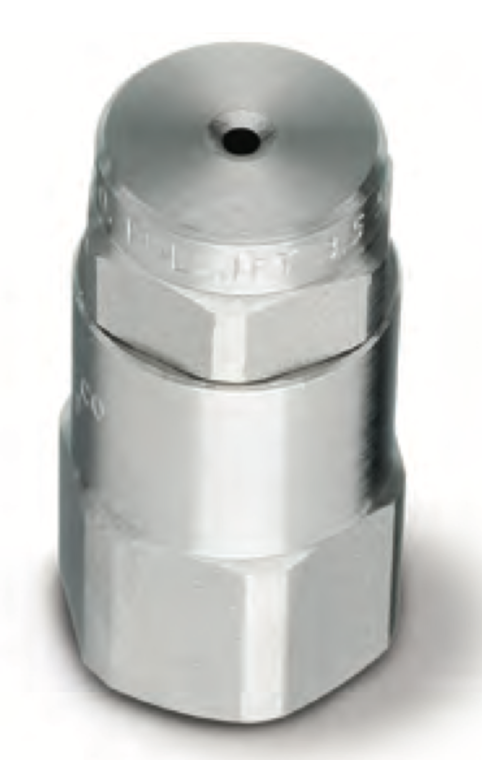
\includegraphics[width = 5cm, height=6cm ]{figures/nzl}
  \caption{Full cone wide angle nozzle}
  \label{fig:nzl}
\end{figure}

** If you wish I can add a detailed description of each variable and the calculation that I did for the selection.\\
\\
Purchased from: Spraying system Canada ltd.\\
\\
Material: Stainless steel 316\\
\\
Part Number: 1/4G-316SS4.3W \\
\\
Important links for product and related literature :
\\
\url{https://www.spray.ca}\\
\\
\url{https://www.spray.com/-/media/DAM/Sales-Materials/b/B652A_Spray_Technology_Dust_Control.pdf}\\
\\
\url{https://www.spray.ca/spray_nozzles/full_cone_fulljet_nozzles.aspx}\\
\\
\url{https://www.spray.ca/literature/literature_cat75.aspx}\\
\\
\url{https://www.spray.ca/Assets/SPRAY/Cat75HYD_US_B.pdf}\\
\\
In our case, we have placed nozzles on the top and bottom to rinse the source thoroughly.\\
\\
\textbf{Bulkhead Fitting and O rings}: \\
\\
\textbf{Bulkhead fitting}:
It is an item that is designed to allow a connection through the wall of a container or vessel. The details of the fittings that we are using are follow:\\
\\
\begin{figure}[!htpb]
  \centering
  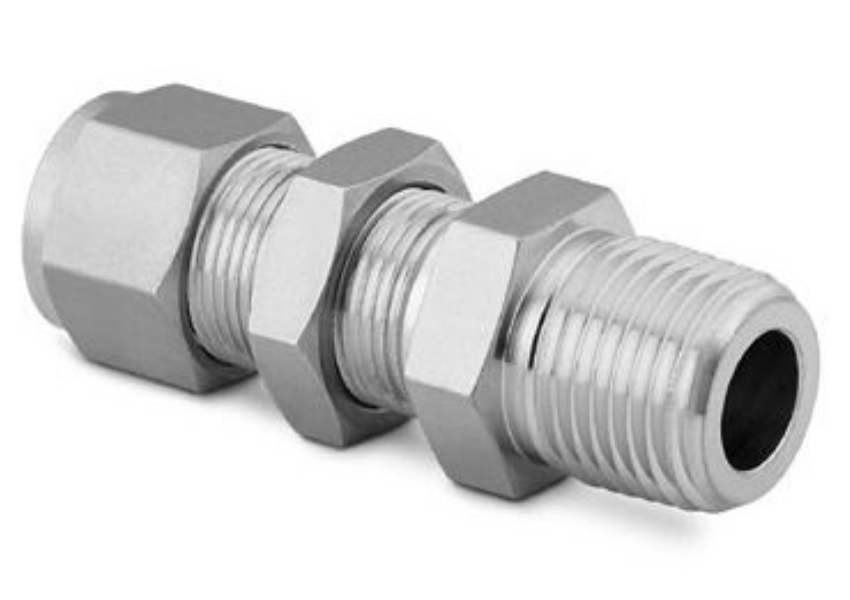
\includegraphics[width = 5cm, height=6cm ]{figures/ftng}
  \caption{Swagelog bulkhead fitting}
  \label{fig:ftng}
\end{figure}
\\
Purchased from: Swagelok Edmonton Valve and Fitting Inc.\\
\\
Material: Stainless steel 316.   \\                           
\\
Part Number: SS-400-11-4\\
\\
 \url{ https://www.swagelok.com/en}\\
\\
Connection type: Bulkhead Male Connector, 1/4$''$Tube OD x 1/4 $''$Male NPT\\
\\
\textbf{O rings}: 
\\
They are commonly used in sealing applications. In our operation we are using chemical resistant Viton Fluoroelastomer O-Ring with the bulkhead fitting for the airtight sealing.\\
\\
Purchased from: McMASTER-CARR.\\
\\
Material: Viton® Fluoroelastomer Rubber\\                                
\\
Part number: 9464K17\\
\\
\url{https://www.mcmaster.com}\\
\\
Technical details: \url{https://www.mcmaster.com/9464k17}\\
\\
\begin{figure}[!htpb]
  \centering
  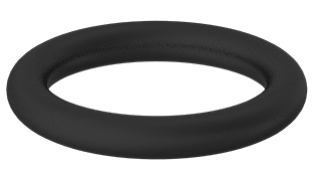
\includegraphics[width = 5cm, height=6cm ]{figures/oring}
  \caption{Viton Fluoroelastomer O-Ring}
  \label{fig:oring}
\end{figure}
\\
\section{ Linear Alkyl Benzene (LAB) cleaning set up}
This setup is designed to clean the LAB. The complete unit consists of different parts such as pump, filters, pulsation dampener, piping system, fitting and cart.  LAB is noncorrosive (SDS) hence doesn’t demand any specific storage but from previous experience and observations, it is recommended to use stainless steel and PTFE wetted parts only, as LAB is known to swell and degrade elastomers over time. \\
\\
\textbf{Parts of LAB set up}:\\
The details of all the parts associated with the unit are as following:\\
\\
\textbf{Piping system and fittings}:\\
\begin{itemize}
\item  1/2$''$ 316 stainless steel tubing with a wall thickness of 0.049$''$: \url{https://www.mcmaster.com/89785k845}.
\end{itemize}

The list of fittings includes:\\
\begin{itemize}
\item Four hose connections (1/2$''$ to 3/8$''$): SS-815-6: \url{ https://www.swagelok.com/en/catalog/Product/Detail?part=SS-815-6}
\end{itemize}

\begin{itemize}
\item Four 1/2$''$ unions: SS-810-6 : \url{https://www.swagelok.com/en/catalog/Product/Detail?part=SS-810-6}
\end{itemize}

\begin{itemize}
\item Five 1/2$''$ MNPT to Female Swagelok Connect: SS-810-1-8 : \url{https://www.swagelok.com/en/catalog/Product/Detail?part=SS-810-1-8}
\end{itemize}

\begin{itemize}
\item One 1/2$''$  MNPT to Male Swagelok connect: SS-8-TA-1-8 : \url{https://www.swagelok.com/en/catalog/Product/Detail?part=SS-8-TA-1-8}
\end{itemize}

\begin{itemize}
\item One 3/4$''$ MNPT to Male Swagelok connect: SS-8-TA-1-12 : \url{https://www.swagelok.com/en/catalog/Product/Detail?part=SS-8-TA-1-12}
\end{itemize}

\begin{itemize}
\item Three   1/2$''$ tees, and one  1/2$''$ tee with a 1/4$''$ connection: SS-810-3: \url{https://www.swagelok.com/en/catalog/Product/Detail?part=SS-810-3}
\end{itemize}

\begin{itemize}
\item Stainless Steel Swagelok Tube Fitting, Male Tube Adapter, 1/4 $''$ Tube OD x 1/4 $''$ Male NPT: SS-4-TA-1-4: \url{https://www.swagelok.com/en/catalog/Product/Detail?part=SS-4-TA-1-4}
\end{itemize}

\begin{itemize}
\item Stainless Steel Swagelok Tube Fitting, Male Tube Adapter, 1/4 $''$  Tube OD x 1/8$''$ Male NPT: SS-4-TA-1-2 : \url{https://www.swagelok.com/en/catalog/Product/Detail?part=SS-4-TA-1-2}
\end{itemize}

\begin{itemize}
\item Stainless Steel Swagelok Tube Fitting, Reducing Union Tee, 1/2 $''$  x 1/2 $''$  x 1/4 $''$ Tube OD: SS-810-3-8-4: \url{https://www.swagelok.com/en/catalog/Product/Detail?part=SS-810-3-8-4}
\end{itemize}

\begin{itemize}
\item One pressure gauge. It has a range from 0 to 100 psi: PGI-63C-OG100-LAQX
\end{itemize} 
\textbf{Valves}: All valves are manufactured by Swagelok and were purchased through Edmonton Valve and Fitting. The list includes:\\
\\
\begin{itemize}
\item Two 3-way 1/2 $''$ valves:SS-45XS8: \url{https://www.swagelok.com/en/catalog/Product/Detail?part=SS-45XS8}
\end{itemize}

\begin{itemize}
\item Two 1/4 $''$valves for the drain ports on the filter housings: SS-42GS4: \url{https://www.swagelok.com/en/catalog/Product/Detail?part=SS-42GS4}\\
\end{itemize} 
\textbf{Pump, Filter, and Pulsation Dampener}\\
\\
\textbf{Air Operated Diaphragm Pump (AODD)}\\
The choice to go with an AODD pump was based on experience from similar wash systems built. Additionally, it is cost effective compared to other pumps and does not require electricity to operate. The Air Operated Double Diaphragm (AODD) pump was manufactured by Sandpiper. It has a housing made out of aluminum and stainless steel and all wetted materials are made up of stainless steel and PTFE. \\
\begin{itemize}
\item \url{https://www.sandpiperpump.com/products/standard-duty-ball/s05-metallic}
\item \url{https://www.mcmaster.com/41655k27}\\
\end{itemize}
The diaphragm and check valve balls are made out of PTFE and the maximum air pressure the pump can handle is 125 psi .The purchased air regulator has an air flow of 53 cfm at 100 psi and has a maximum pressure of 140 psi.\\
\url{ https://www.mcmaster.com/8812k52.}\\
A performance curve of the pump can be found here : \url{https://www.sandpiperpump.com/products/standard-duty-ball/s05-metallic}.\\
 \\
 \textbf{Filter Housing}\\
To not impede the flow rate of the fluid, 20$''$ long filter housings have purchased and to accommodate the filters, two stainless steel Shelco 20$''$  Filter housings have procured through CPS Filtration. They are designed for a 20$''$ (length) and 2.5$''$  (diameter) filter cartridge.\\
\url{ https://cpsfiltration.com}\\
\\
\textbf{Filter Cartridge}\\
The cartridges are made up of 20$''$ PTFE membrane with polypropylene core material and Teflon (PTFE) gaskets.  The filter cartridges were purchased through CPS filtration and  are manufactured by American Melt Blown and Filtration. They have a maximum differential pressure of 45 psid (pounds per square inch differential).\\
\url{  https://cpsfiltration.com}\\
\\
\textbf{Pulsation Dampener}\\
One disadvantage to using an AODD pump, is that the pressure of the fluid is periodic, since the pump pulses due to the diaphragms opening and closing. The pulsation dampener is designed to correct this by “smoothing” out the pulsations of the fluid, so that a laminar flow is achieved. The pulsation dampener was manufactured by Blacoh(\url{https://www.blacoh.com/home.aspx}) Fluid Control and  model CT3120T was purchased through Natpro. The pulsation dampener is made out of stainless steel with a PTFE bladder.  It hold a maximum operating pressure 300 psi at \ang{20} C. The pulsation dampener must be charged to 80$\%$ of the head pressure to ensure maximal dampening.\\
\\
\textbf{Cart Framing}\\
Made out of 1.5” T-Slot Aluminum extrusions (manufactured by 8020) due to its ease of assembly and versatility. 
\url{https://8020.net/?SID=og9et35936f61t6v13tron8os1}
\url{https://www.mcmaster.com/47065t103}    \\
\\
\textbf{Spill Tray}
\begin{itemize}
\item Made out of polypropylene:\url{https://www.usplastic.com/catalog/item.aspx?itemid=125655}
\item Dimension: 24$''$x24$''$x4$''$
\item Can hold 37 litres of fluid
\end{itemize}



 














